\documentclass{beamer}
\usetheme{Boadilla}
\usepackage{enumitem}
\usepackage{graphicx}
%\usepackage[retainorgcmds]{IEEEtrantools}
%\setbeamertemplate{enumerate items}[ball]

\title{Speculative Synchronization in StarSs, a task-based Programming Model}
\subtitle{PhD and the current Work}
\author{Rahul}
\date{\today}

\usepackage[utf8]{ inputenc}
\usepackage{default}

\begin{document}

\begin{frame}
 \titlepage
\end{frame}

\begin{frame}
 \frametitle{Outline}
 \tableofcontents
\end{frame}


\section{Introduction to StarSs}

%%%%%%%%%%%%%%%%%%%%%%
\begin{frame}

\frametitle{Introduction to StarSs}

  \begin{itemize}
   \item An implicit parallel programming model for widely used multi-core architectures
   \item Sequential application code with pragmas
   \item \textbf{pragmas} - compiler directives to mark tasks (a block of code)
   \item Data-dependency analysis between tasks is performed by the StarSs runtime
   \begin{itemize}
    \item Task Dependency Graph (TDG)
   \end{itemize}
  \end{itemize}
  
\end{frame}
%%%%%%%%%%%%%%%%%%%%%%

 \begin{frame}
 
\frametitle{StarSs runtime features}

\begin{columns}
 
 \column{0.5\textwidth}
 \begin{itemize}
  \item Main thread of Control
  \item Worker Threads
  \end{itemize}
  
 \column{0.5\textwidth}
  \begin{figure}
  \centering
   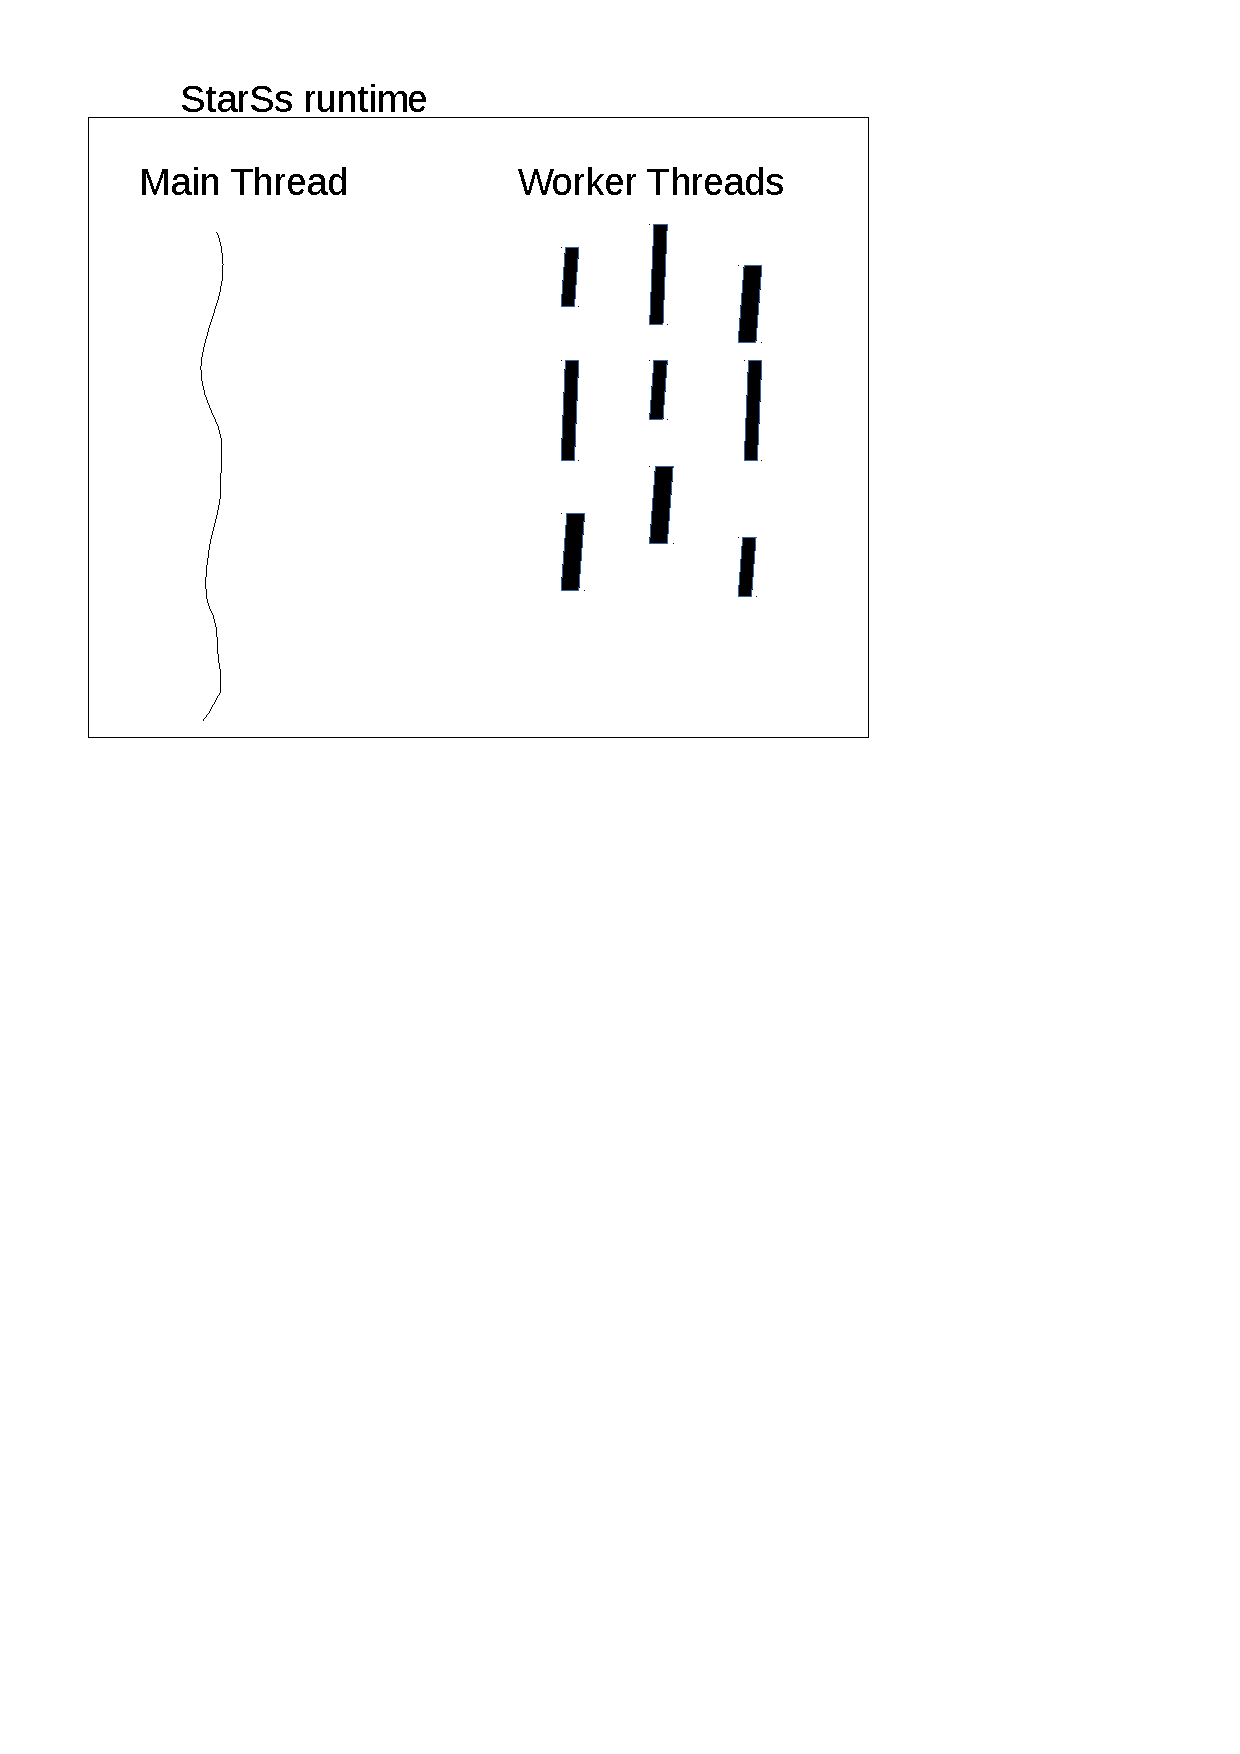
\includegraphics[scale=0.5]{StarSs-runtime.pdf}
  \end{figure}


\end{columns}
  
\end{frame}
%%%%%%%%%%%%%%%%%%%%%%

% \begin{frame}
% 
% \frametitle{StarSs Runtime}
%   
% \end{frame}
% %%%%%%%%%%%%%%%%%%%%%%
% 
% \begin{frame}
% 
% \frametitle{Need for Synchronization}
%   
% \end{frame}
% 
% %%%%%%%%%%%%%%%%%%%%%%%%%%%%%%%%%%section STM %%%%%%%%%%%%%%%%%%%%%%%%%%%%%%%%
% 
% \section{Software Transactional Memory (STM)}
% 
% \begin{frame}
% 
%  \frametitle{Software Transactional Memory (STM)}
%  
% \end{frame}
% %%%%%%%%%%%%%%%%%%%%%%
% 
% \begin{frame}
% 
% \frametitle{Locks versus STM}
% 
% \end{frame}
% 
% %%%%%%%%%%%%%%%%%%%%%%%%%%%%%%%%%%Conclusion %%%%%%%%%%%%%%%%%%%%%%%%%%%%%%%%
% 
% \section{Conclusion}
% 
% \begin{frame}
% 
% \frametitle{Conclusion}
% 
% \end{frame}



\end{document}
